\iffalse
\let\negmedspace\undefined
\let\negthickspace\undefined
\documentclass[journal,12pt,onecolumn]{IEEEtran}
\usepackage{cite}
\usepackage{amsmath,amssymb,amsfonts,amsthm}
\usepackage{algorithmic}
\usepackage{graphicx}
\usepackage{textcomp}
\usepackage{xcolor}
\usepackage{txfonts}
\usepackage{listings}
\usepackage{enumitem}
\usepackage{mathtools}
\usepackage{gensymb}
\usepackage{comment}
\usepackage[breaklinks=true]{hyperref}
\usepackage{tkz-euclide} 
\usepackage{listings}
\usepackage{gvv}                                        
\def\inputGnumericTable{}                                 
\usepackage[latin1]{inputenc}                                
\usepackage{color}                                            
\usepackage{array}                                            
\usepackage{longtable}                                       
\usepackage{calc}                                             
\usepackage{multirow}                                         
\usepackage{hhline}                                           
\usepackage{ifthen}                                           
\usepackage{lscape}
\usepackage{caption}

\newtheorem{theorem}{Theorem}[section]
\newtheorem{problem}{Problem}
\newtheorem{proposition}{Proposition}[section]
\newtheorem{lemma}{Lemma}[section]
\newtheorem{corollary}[theorem]{Corollary}
\newtheorem{example}{Example}[section]
\newtheorem{definition}[problem]{Definition}
\newcommand{\BEQA}{\begin{eqnarray}}
\newcommand{\EEQA}{\end{eqnarray}}
\newcommand{\define}{\stackrel{\triangle}{=}}
\theoremstyle{remark}
\newtheorem{rem}{Remark}
\begin{document}

\bibliographystyle{IEEEtran}
\vspace{3cm}

\title{10.5.4}
\author{EE23BTECH11029 - Kanishk}
\maketitle

\bigskip

\renewcommand{\thefigure}{\theenumi}
\renewcommand{\thetable}{\theenumi}
\textbf{Question}:\\
The houses of a row are numbered consecutively from 1 to 49. Show that there is a value
of x such that the sum of the numbers of the houses preceding the house numbered is equal to the sum of the numbers of the houses following it. Find this value of $x$.\\
Hint:$ S_{x-1}=S_{49}-S_x$

\textbf{Solution}:\\
\fi
\begin{table}[ht]
    \centering
    \def\arraystretch{2.5}
    \footnotesize
\begin{tabular}{|c|c|c|}
\hline
Parameter & Value & Description \\
\hline
$x\brak{0}$ & $1$ & First house \\
\hline
$d$ & $1$ & Common difference\\
\hline
$x\brak{n}$ & $\brak{n+1}u\brak{n}$ & $\brak{n+1}th$ house\\
\hline
$y\brak{n}$ & $\brak{\frac{n+1}{2}}\brak{n+2}u\brak{n}$ & Sum of $n+1$ number of houses.\\
\hline
$x_2\brak{n}$ & $\brak{49-n}u\brak{n}$ & $\brak{n+1}th$ house from last house\\
\hline
$y_2\brak{n}$ & $\sbrak{49n-\brak{\frac{n}{2}}\brak{n+1}}u\brak{n}$ & Sum of $n+1$ houses from last house.\\
\hline
\end{tabular}
   \caption{Input Parameters}
   \label{tab:10.5.4}
\end{table}

For an AP: 
\begin{align}
X\brak{z}&=\frac{x\brak{0}}{1-z^{-1}}+ \frac{dz^{-1}}{\brak{1-z^{-1}}^{2}}\\
\implies X\brak{z}&=\frac{1}{1-z^{-1}}+ \frac{z^{-1}}{\brak{1-z^{-1}}^{2}}\\
&=\frac{1}{\brak{1-z^{-1}}^{2}},\quad \abs{z} > 1
\end{align}

\begin{align}
    \therefore y\brak{n}=\frac{\brak{n+1}}{2}\brak{n+2}
\end{align}

\begin{align}
y\brak{x-2}&=y\brak{n-1}-y\brak{x-1}
\end{align}

\newpage
From \tabref{tab:10.5.4}:

\begin{align}
\brak{\frac{x-1}{2}}x&=\frac{n}{2}\brak{n+1}-\frac{x}{2}\brak{x+1}\\
\brak{x-1}+x\brak{x+1}&=n\brak{n+1}\\
2x^{2}&=n\brak{n+1}\\
x&=\sqrt{\frac{n}{2}\brak{n+1}}\\
x&=35
\end{align}

\textbf{Result Confirmation:}\\

To prove:\\
\begin{equation}
y\brak{33}=y_2\brak{13}
\end{equation}

\textbf{LHS:}\\

\begin{align}
y\brak{n}&=x\brak{n}*u\brak{n}\\
\implies Y\brak{z}&=X\brak{z} \times U\brak{z}\\
Y\brak{z}&=\brak{\frac{1}{\brak{1-z^{-1}}^2}}\brak{\frac{1}{1-z^{-1}}}\\
&=\frac{1}{\brak{1-z^{-1}}^3},\quad \abs{z}>1\\
\end{align}

Using Contour Integration to find inverse Z-transform,

\begin{align}
y\brak{33}&=\frac{1}{2\pi j}\oint_{C}Y(z) \;z^{32} \;dz\\
 &=\frac{1}{2\pi j}\oint_{C}\frac{z^{32}}{({1-z^{-1})}^{3}} \;dz 
\end{align}
We can observe that the pole is repeated $3$ times and thus $m=3$,

\begin{align}
R&=\frac{1}{\brak {m-1}!}\lim\limits_{z\to a}\frac{d^{m-1}}{dz^{m-1}}\brak {{(z-a)}^{m}f\brak z} \\
&=\frac{1}{\brak {2}!}\lim\limits_{z\to 1}\frac{d^{2}}{dz^{2}}\brak{z^{35}}\\
&=595
\end{align}

\newpage
\textbf{RHS:}\\

\quad From \tabref{tab:10.5.4}:

\begin{align}
X_2\brak{z}&=\frac{49-50z^{-1}}{\brak{1-z^{-1}}^{2}}\\
y_2\brak{n}&=x_2\brak{n}*u\brak{n}\\
\implies Y_2\brak{z}&=X_2\brak{z} \times U\brak{z}\\
y_2\brak{z}&=\frac{49-50z^{-1}}{\brak{1-z^{-1}}^{3}}\\
\end{align}

Using Contour Integration to find inverse Z-transform,
\begin{align}
y_2\brak{13}&=\frac{1}{2\pi j}\oint_{C}Y(z) \;z^{12} ;dz\\
 &=\frac{1}{2\pi j}\oint_{C}\frac{49-50z^{-1}}{({1-z^{-1})}^{3}}\brak{z^{12}} \;dz 
\end{align}

We can observe that the pole is repeated $3$ times and thus $m=3$,

\begin{align}
R&=\frac{1}{\brak {m-1}!}\lim\limits_{z\to a}\frac{d^{m-1}}{dz^{m-1}}\brak {{(z-a)}^{m}f\brak z} \\
&=\frac{1}{\brak {2}!}\lim\limits_{z\to 1}\frac{d^{2}}{dz^{2}}\brak{49z^{15}-50z^{14}}\\
&=49.15.14-50.14.13\\
&=595
\end{align}
\[ LHS = RHS \]




\begin{figure}[h]
    \centering
    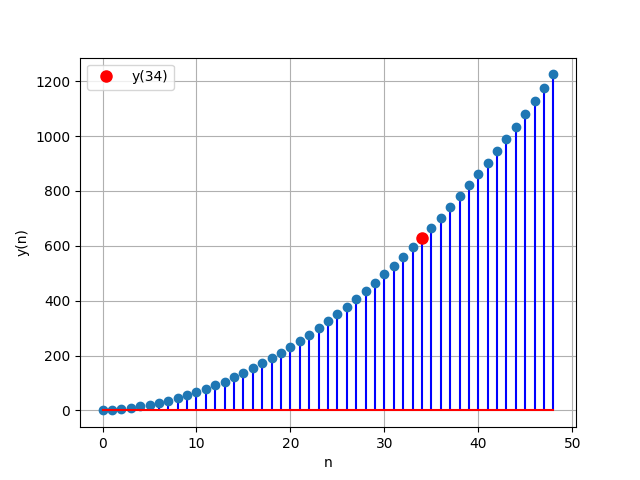
\includegraphics[width=100mm]{ncert-maths/10/5/4/4/figs/fig1.png}
    \caption{Plot y(n) vs n}
\end{figure}

% \end{document}